\documentclass[11pt,a4paper]{report}

% Essential packages
\usepackage[utf8]{inputenc}
\usepackage[T1]{fontenc}
\usepackage{lmodern} % Modern fonts
\usepackage{microtype} % Better typography
\usepackage{geometry}
\usepackage{graphicx}
\usepackage{xcolor}
\usepackage{tikz}
\usepackage{pgfplots}
\usepackage{booktabs}
\usepackage{tabularx}
\usepackage{longtable}
\usepackage{multirow}
\usepackage{array}
\usepackage{hyperref}
\usepackage{fancyhdr}
\usepackage{titlesec}
\usepackage{tocloft}
\usepackage{enumitem}
\usepackage{amsmath}
\usepackage{amssymb}
\usepackage{caption}
\usepackage{subcaption}
\usepackage{float}
\usepackage{wrapfig}
\usepackage{lipsum}
\usepackage{etoolbox}
\usepackage{afterpage}
\usepackage[most]{tcolorbox}

% Page geometry
\geometry{
    left=25mm,
    right=25mm,
    top=30mm,
    bottom=30mm,
    headheight=15pt
}
% Color scheme - theBlockchain.ai brand palette
\definecolor{ocean}{RGB}{0, 123, 255}        % Ocean (Blue) - Primary brand color
\definecolor{sky}{RGB}{23, 162, 184}         % Sky (Cyan) - Secondary brand color
\definecolor{sun}{RGB}{253, 126, 20}         % Sun (Orange) - Accent brand color
\definecolor{trust}{RGB}{40, 167, 69}        % Trust (Green) - Success brand color
\definecolor{darkgray}{RGB}{52, 58, 64}      % Dark neutral
\definecolor{lightgray}{RGB}{248, 249, 250}  % Light neutral
% Legacy aliases for compatibility
\definecolor{primaryblue}{RGB}{0, 123, 255}
\definecolor{secondaryblue}{RGB}{23, 162, 184}
\definecolor{accentgreen}{RGB}{40, 167, 69}
\definecolor{warnorange}{RGB}{253, 126, 20}

% TikZ libraries
\usetikzlibrary{shapes,arrows,positioning,calc,shadows.blur,decorations.pathreplacing}
\pgfplotsset{compat=1.18}

% Header and footer styling
\pagestyle{fancy}
\fancyhf{}
\fancyhead[L]{\footnotesize\textcolor{darkgray}{The Convergent Economy}}
\fancyhead[R]{\footnotesize\textcolor{darkgray}{\thepage}}
\renewcommand{\headrulewidth}{0.5pt}
\renewcommand{\footrulewidth}{0pt}

% Chapter and section formatting
\titleformat{\chapter}[display]
{\normalfont\huge\bfseries\color{ocean}}
{\textcolor{sun}{\chaptertitlename\ \thechapter}}{20pt}{\Huge\color{ocean}}

\titleformat{\section}
{\normalfont\Large\bfseries\color{sky}}{\textcolor{sun}{\thesection}}{1em}{}

\titleformat{\subsection}
{\normalfont\large\bfseries\color{darkgray}}
{\thesubsection}{1em}{}
% Table of contents formatting
\renewcommand{\cftchapfont}{\bfseries\color{ocean}}
\renewcommand{\cftsecfont}{\color{sky}}
\renewcommand{\cftsubsecfont}{\color{trust}}

% Custom environments
\newtcolorbox{keypoint}[1][]{
    enhanced,
    before skip=10pt,
    after skip=10pt,
    colback=lightgray,
    colframe=primaryblue,
    boxrule=2pt,
    left=10pt,
    right=10pt,
    top=10pt,
    bottom=10pt,
    sharp corners,
    title={#1},
    coltitle=white,
    fonttitle=\bfseries,
}

\newtcolorbox{marketfigure}[1][]{
    colback=trust!5,
    colframe=trust,
    fonttitle=\bfseries\color{trust},
    title=#1,
    boxrule=2pt,
    arc=2pt,
    attach boxed title to top center={yshift=-3mm},
    boxed title style={colback=sun!20, colframe=sun, boxrule=1pt}
}

% Custom commands with brand colors
\newcommand{\marketvalue}[2]{\textcolor{trust}{\textbf{\$#1}}\,\textcolor{darkgray}{#2}}
\newcommand{\cagr}[1]{\textcolor{sun}{\textbf{#1\%}}}
\newcommand{\techterm}[1]{\textbf{\textcolor{ocean}{#1}}}

% Hyperref setup with brand colors
\hypersetup{
    colorlinks=true,
    linkcolor=ocean,
    filecolor=sky,
    urlcolor=sun,
    citecolor=trust,
    pdftitle={The Convergent Economy: Market Analysis of AI, Software, and Blockchain},
    pdfauthor={},
    pdfsubject={Technology Market Analysis},
    pdfkeywords={AI, Blockchain, Software Development, Tokenization, Digital Assets}
}

\begin{document}

% Title page
\begin{titlepage}
    \begin{tikzpicture}[remember picture,overlay]
        % Multi-color gradient background
        \shade[top color=sky!20, bottom color=ocean!10] (current page.north west) rectangle (current page.south east);
        
        % Brand color decorative elements
        \foreach \i in {1,...,5}{
            \pgfmathsetmacro{\colorintensity}{\i*20}
            \node[circle, draw=sun!\colorintensity, line width=\i pt, minimum size=\i cm] 
                at ($(current page.north east) + (-3,-3)$) {};
        }
        
        % Additional decorative elements with brand colors
        \foreach \i in {1,...,3}{
            \pgfmathsetmacro{\colorintensity}{\i*30}
            \node[circle, draw=trust!\colorintensity, line width=\i pt, minimum size=\i cm] 
                at ($(current page.north west) + (3,-3)$) {};
        }
        
        % Enhanced network visualization with brand colors
        \begin{scope}[shift={($(current page.center)+(0,3)$)}]
            % AI node - Ocean (Blue)
            \node[circle, fill=ocean, text=white, font=\bfseries, 
                  minimum size=1.5cm, blur shadow] 
                (node0) at (0:3cm) {AI};
            % Software node - Sky (Cyan)
            \node[circle, fill=sky, text=white, font=\bfseries, 
                  minimum size=1.5cm, blur shadow] 
                (node120) at (120:3cm) {Software};
            % Blockchain node - Sun (Orange)
            \node[circle, fill=sun, text=white, font=\bfseries, 
                  minimum size=1.5cm, blur shadow] 
                (node240) at (240:3cm) {Blockchain};
            
            % Connecting lines with gradient colors
            \draw[ocean!70, line width=3pt] (node0) -- (node120);
            \draw[sky!70, line width=3pt] (node120) -- (node240);
            \draw[sun!70, line width=3pt] (node240) -- (node0);
            
            % Central TOKEN node - Trust (Green)
            \node[circle, fill=trust, text=white, font=\bfseries\small,
                  minimum size=1.2cm, blur shadow] at (0,0) {TOKEN};
        \end{scope}
    \end{tikzpicture}
    
    \vspace*{2cm}
    
    \begin{center}
        {\Huge\bfseries\color{ocean} The Convergent Economy}\\[0.5cm]
        {\Large\color{sky} Market Analysis of \textcolor{ocean}{AI}, \textcolor{sky}{Software}, and \textcolor{sun}{Blockchain}}\\[0.3cm]
        {\Large\color{trust} and the Unifying Role of \textcolor{sun}{Tokenization}}\\[2cm]
        
        \begin{tcolorbox}[
            width=0.8\textwidth,
            colback=sky!5,
            colframe=ocean,
            boxrule=3pt,
            arc=0pt,
            outer arc=0pt
        ]            \centering\large
            \textbf{Executive Report}\\[0.5cm]
            Analyzing the \marketvalue{5+ Trillion}{} Opportunity\\
            at the Intersection of Three Revolutionary Technologies
        \end{tcolorbox}
        
        \vfill
        
        {\large\color{darkgray}\today}
    \end{center}
\end{titlepage}

% Table of Contents
\tableofcontents

% Executive Summary
\chapter*{Executive Summary}
\addcontentsline{toc}{chapter}{Executive Summary}

\begin{keypoint}[Key Thesis]
Tokenization is the fundamental economic and trust layer that will unlock the multi-trillion-dollar potential of the convergent AI, software, and blockchain economy.
\end{keypoint}

The global technology landscape is on the cusp of a paradigm shift, driven by the convergence of three powerful, independently massive forces: Artificial Intelligence (AI), software development, and blockchain technology. While each market represents a trillion-dollar opportunity in its own right, their intersection creates a novel economic frontier characterized by intelligent, autonomous systems and new models of value creation and exchange.

\section*{Market Overview}
The analysis reveals that the standalone markets for AI, software, and blockchain are projected to collectively command a value well in excess of \marketvalue{5 trillion}{} by the early 2030s. The nascent ``Blockchain AI'' market, though smaller in absolute terms today, is expanding at a compound annual growth rate (CAGR) approaching \cagr{40}, indicating a significant market premium for AI systems enhanced with blockchain's inherent trust and security features.

\begin{marketfigure}[Market Figures at a Glance]
\centering
\begin{tabular}{lrrr}
\toprule
\textbf{Market Sector} & \textbf{2025 Size} & \textbf{2034 Forecast} & \textbf{CAGR} \\
& (USD Billion) & (USD Billion) & \\
\midrule
Artificial Intelligence & \marketvalue{757.58}{} & \marketvalue{3,680.47}{} & \cagr{19.20} \\
Custom Software Dev. & \marketvalue{53.02}{} & \marketvalue{334.49}{} & \cagr{22.71} \\
Blockchain Technology & \marketvalue{31.18}{} & \marketvalue{393.42}{} & \cagr{43.60} \\
Blockchain AI & \marketvalue{1.12}{} & \marketvalue{5.38}{} & \cagr{37.18} \\
\bottomrule
\end{tabular}
\end{marketfigure}

This convergence is not merely additive; it is symbiotic. Blockchain provides a verifiable, immutable foundation that solves AI's ``black box'' problem, while AI optimizes and secures blockchain operations.

\section*{The Output: A New Asset Class}
The output of this convergence is a new class of digital asset: autonomous AI agents, dynamic software modules, and decentralized, self-governing ecosystems. Traditional models of ownership, licensing, and monetization are inadequate for these fluid, intelligent assets. 

\techterm{Tokenization}, particularly through versatile standards like ERC-1155, provides the comprehensive solution. It enables:

\begin{itemize}[leftmargin=2cm]
    \item[$\bullet$] Fractionalization of ownership
    \item[$\bullet$] Creation of liquid secondary markets for previously illiquid IP
    \item[$\bullet$] Automation of royalty streams via smart contracts
    \item[$\bullet$] Establishment of decentralized, token-governed software projects
\end{itemize}

\section*{Strategic Outlook}

This report offers a strategic outlook for investors, executives, and founders, identifying key growth sectors. The most significant near-term opportunities lie in horizontal, enabling infrastructure, including:

\begin{enumerate}
    \item \textbf{Tokenization-as-a-Service (TaaS) platforms}
    \item \textbf{Enhanced AI model training} through blockchain-verified datasets
    \item \textbf{Decentralized AI marketplaces} with tokenized model ownership
    \item \textbf{Smart contract automation} for AI service agreements
\end{enumerate}

While regulatory uncertainty remains the most significant headwind, the trajectory is clear. The convergence of AI, software, and blockchain, unified by tokenization, is paving the way for a more transparent, efficient, and liquid global digital economy.
% Chapter 1
\chapter{The Trillion-Dollar Triumvirate: Sizing the Foundational Markets}

To comprehend the magnitude of the convergent opportunity, it is first necessary to establish the immense, independent scale of the three core technology pillars. Artificial Intelligence, software development, and blockchain each represent massive global markets with distinct growth dynamics. Their individual trajectories provide the foundational context for the powerful economic gravity they exert upon one another.

\section{The Artificial Intelligence Market: A Multi-Trillion Dollar Future}

The global AI market is undergoing a period of explosive growth, transforming virtually every industry with enhanced data analysis, automation, and operational efficiency. While forecasts vary based on scope and methodology, they consistently point toward a market valued in the trillions of dollars within the next decade.

\begin{figure}[H]
\centering
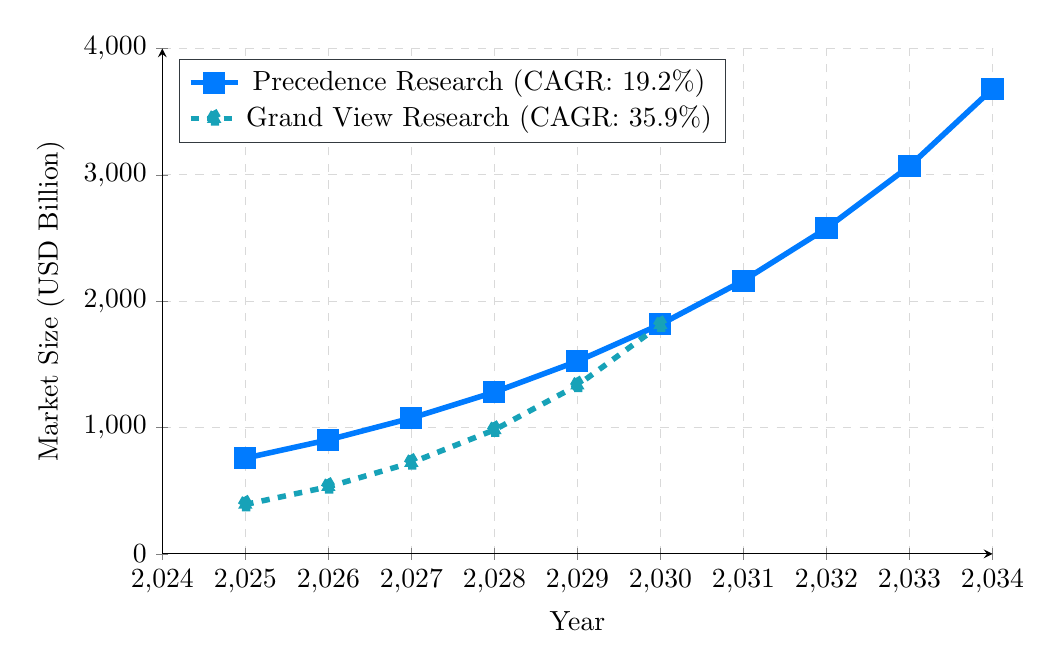
\begin{tikzpicture}
\begin{axis}[
    width=\textwidth,
    height=8cm,
    xlabel={Year},
    ylabel={Market Size (USD Billion)},
    xmin=2024, xmax=2034,
    ymin=0, ymax=4000,
    xtick={2024,2025,2026,2027,2028,2029,2030,2031,2032,2033,2034},
    legend pos=north west,
    grid=major,
    grid style={dashed,gray!30},
    axis lines=left,
    legend style={at={(0.02,0.98)},anchor=north west,fill=white,draw=darkgray}
]% Precedence Research projection
\addplot[
    color=primaryblue,
    line width=2pt,
    mark=square*,
    mark options={scale=1.5}
] coordinates {
    (2025,757.58)
    (2026,902.41)
    (2027,1074.67)
    (2028,1279.91)
    (2029,1524.61)
    (2030,1816.21)
    (2031,2163.10)
    (2032,2576.41)
    (2033,3069.01)
    (2034,3680.47)
};
\addlegendentry{Precedence Research (CAGR: 19.2\%)}

% Grand View Research projection
\addplot[
    color=secondaryblue,
    line width=2pt,
    mark=triangle*,
    mark options={scale=1.5},
    dashed
] coordinates {
    (2025,390.91)
    (2026,531.33)
    (2027,721.96)
    (2028,981.38)
    (2029,1334.14)
    (2030,1811.75)
};
\addlegendentry{Grand View Research (CAGR: 35.9\%)}
\end{axis}
\end{tikzpicture}
\caption{AI Market Growth Projections from Leading\\Research Firms}
\end{figure}
\subsection{Market Composition and Drivers}

Precedence Research calculates the AI market at \marketvalue{757.58 billion}{} in 2025, projecting it will soar to \marketvalue{3.68 trillion}{} by 2034, reflecting a robust compound annual growth rate (CAGR) of \cagr{19.20}. Grand View Research presents an even more aggressive short-term forecast, estimating the market will grow from \marketvalue{390.91 billion}{} in 2025 to \marketvalue{1.81 trillion}{} by 2030, driven by a remarkable CAGR of \cagr{35.9}.

\begin{keypoint}[Investment Surge]
Global corporate investment in AI has reached \marketvalue{252 billion}{}, a thirteen-fold increase since 2014, with 92\% of companies planning to increase their AI investments in the next three years.
\end{keypoint}

The market's composition is diversified across technology, solutions, and end-users:

\begin{itemize}
    \item \textbf{Deep learning} stands as the dominant technology, accounting for a 37.4\% market share in 2024
    \item The \textbf{services segment} emerges as the leader, contributing over 39.2\% of revenue in 2024
    \item The \textbf{BFSI sector} is a major adopter, holding a 17.4\% share in 2024
\end{itemize}

\subsection{Geographic Distribution}
\begin{wrapfigure}{r}{0.5\textwidth}
\centering
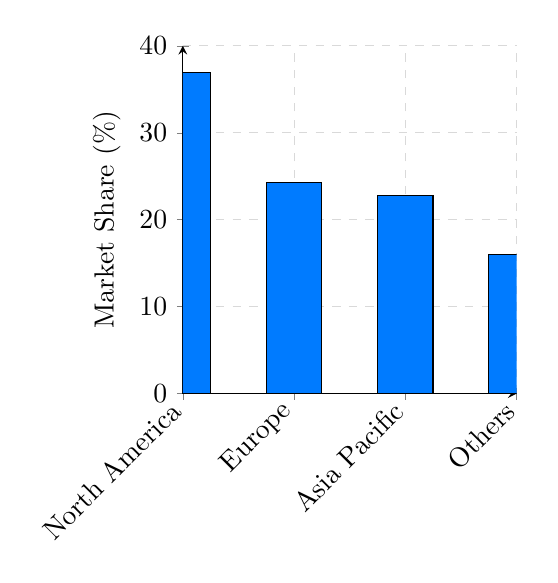
\begin{tikzpicture}
\begin{axis}[
    width=0.48\textwidth,
    height=6cm,
    ybar,
    bar width=20pt,
    ylabel={Market Share (\%)},
    symbolic x coords={North America, Europe, Asia Pacific, Others},
    xtick=data,
    x tick label style={rotate=45,anchor=east},
    ymin=0,
    ymax=40,
    grid=major,
    grid style={dashed,gray!30},
    axis lines=left
]
\addplot[fill=primaryblue] coordinates {
    (North America,36.92)
    (Europe,24.3)
    (Asia Pacific,22.8)
    (Others,15.98)
};
\end{axis}
\end{tikzpicture}
\caption{Global AI Market Share by Region\\(2024)}
\end{wrapfigure}

Geographically, North America leads the global AI market, having captured over 36.92\% of the total market share in 2024. This dominance is propelled by massive private funding in the United States, which at \marketvalue{109.1 billion}{} in 2024, was 12 times that of China. 

The U.S. AI market alone is projected to grow from \marketvalue{146.09 billion}{} in 2024 to \marketvalue{851.46 billion}{} by 2034.

Concurrently, the Asia Pacific region is forecast to be the fastest-growing market, with a projected CAGR of \cagr{19.8} between 2025 and 2034.

\section{The Blockchain Infrastructure Market: Beyond Cryptocurrency}

The blockchain market, while the smallest of the three pillars in absolute terms, is characterized by exponential growth rates, signaling its position in the early, high-growth phase of its adoption cycle.
\begin{table}[H]
\centering
\caption{Blockchain Market Growth Projections}
\begin{tabular}{lcccc}
\toprule
\textbf{Research Firm} & \textbf{2025} & \textbf{End Year} & \textbf{Forecast} & \textbf{CAGR} \\
& (USD Bn) & & (USD Bn) & \\
\midrule
Fortune Business Insights & 31.18 & 2032 & 393.42 & \cagr{43.6} \\
Grand View Research & 57.72 & 2030 & 1,431.54 & \cagr{90.1} \\
\bottomrule
\end{tabular}
\end{table}

This explosive growth is driven by the technology's expanding utility far beyond its origins in cryptocurrency. The market's composition reflects this shift toward foundational utility:

\begin{itemize}
    \item The \textbf{Infrastructure \& Protocols segment} dominated the market in 2024
    \item \textbf{Blockchain-as-a-Service (BaaS)} captured the largest share of the component market
    \item North America held a \textbf{43.65\% share} in 2024
\end{itemize}

\subsection{Comparative Market Analysis}

\begin{keypoint}[Growth Rate Disparity]
The CAGRs for blockchain (43-90\%) substantially exceed those for AI (19-36\%) and software development (13-23\%), indicating blockchain's position at an earlier point on its adoption S-curve.
\end{keypoint}

This disparity suggests that blockchain is at a much earlier point on its adoption S-curve. For investors and strategists, this signals a higher-risk, higher-reward environment. The immense, established total addressable markets (TAMs) of AI and software act as a powerful gravitational force, suggesting that the most valuable near-term blockchain applications will be those that service these existing behemoth industries.

\subsection{Quantifying the Convergence Market}

The specific ``Blockchain AI'' market, though nascent, is already being tracked by analysts and shows a trajectory of hyper-growth:

\begin{table}[H]
\centering
\caption{Blockchain AI Market Projections}
\begin{tabular}{lccc}
\toprule
\textbf{Research Firm} & \textbf{2024 Size} & \textbf{2030 Forecast} & \textbf{CAGR} \\
& (USD Million) & (USD Billion) & \\
\midrule
Research and Markets & 808.13 & 5.38 & \cagr{37.18} \\
Market Research Future & 3,320 & 70.0 (by 2035) & -- \\
\bottomrule
\end{tabular}
\end{table}

A critical observation is that the projected CAGRs for the Blockchain AI market (ranging from 28\% to 37\%) are consistently higher than the standalone AI market's growth rates. This delta suggests a significant ``value-add'' premium.

\clearpage
\section{The Global Software Development Engine:\\Scale, Growth, and Cloud Dominance}

The software development market is a mature, yet continuously expanding cornerstone of the global economy. Market intelligence values the market at \marketvalue{0.57}{trillion} in 2024, forecasting it to reach \marketvalue{1.04}{trillion} by 2030 at a steady CAGR of \cagr{12.90}.

\subsection{Custom Software Development: The High-Growth Segment}
Within this vast landscape, the custom software development segment is experiencing particularly rapid growth. This sector, focused on creating bespoke solutions for specific enterprise needs, is projected to expand from \marketvalue{53.02}{billion} in 2025 to \marketvalue{334.49}{billion} by 2034, accelerating at a CAGR of \cagr{22.71}.

\subsection{Geographic Distribution}
Geographically, North America leads the global AI market, having captured over 36.92\% of the total market share in 2024. This dominance is propelled by massive private funding in the United States, which at \marketvalue{109.1}{billion} in 2024, was 12 times that of China.

The U.S. AI market alone is projected to grow from \marketvalue{146.09}{billion} in 2024 to \marketvalue{51.6}{billion} by 2034.

Concurrently, the Asia Pacific region is forecast to be the fastest-growing market, with a projected CAGR of \cagr{19.8} between 2025 and 2034.

% Chapter 2
\chapter{The Convergence Catalyst: A New Economic Frontier}

The true transformative potential lies not within the individual silos of AI, software, and blockchain, but at their intersection. This convergence is creating a new economic frontier, a specific and quantifiable market where these technologies are not just coexisting but are symbiotically enhancing one another to create novel forms of value.

\section{Synergies and Symbiosis: How AI and Blockchain Mutually Reinforce Value}

The relationship between AI and blockchain is mutually reinforcing, with each technology addressing the inherent weaknesses of the other. This synergy is the primary catalyst for the new market's emergence.

\begin{figure}[H]
\centering
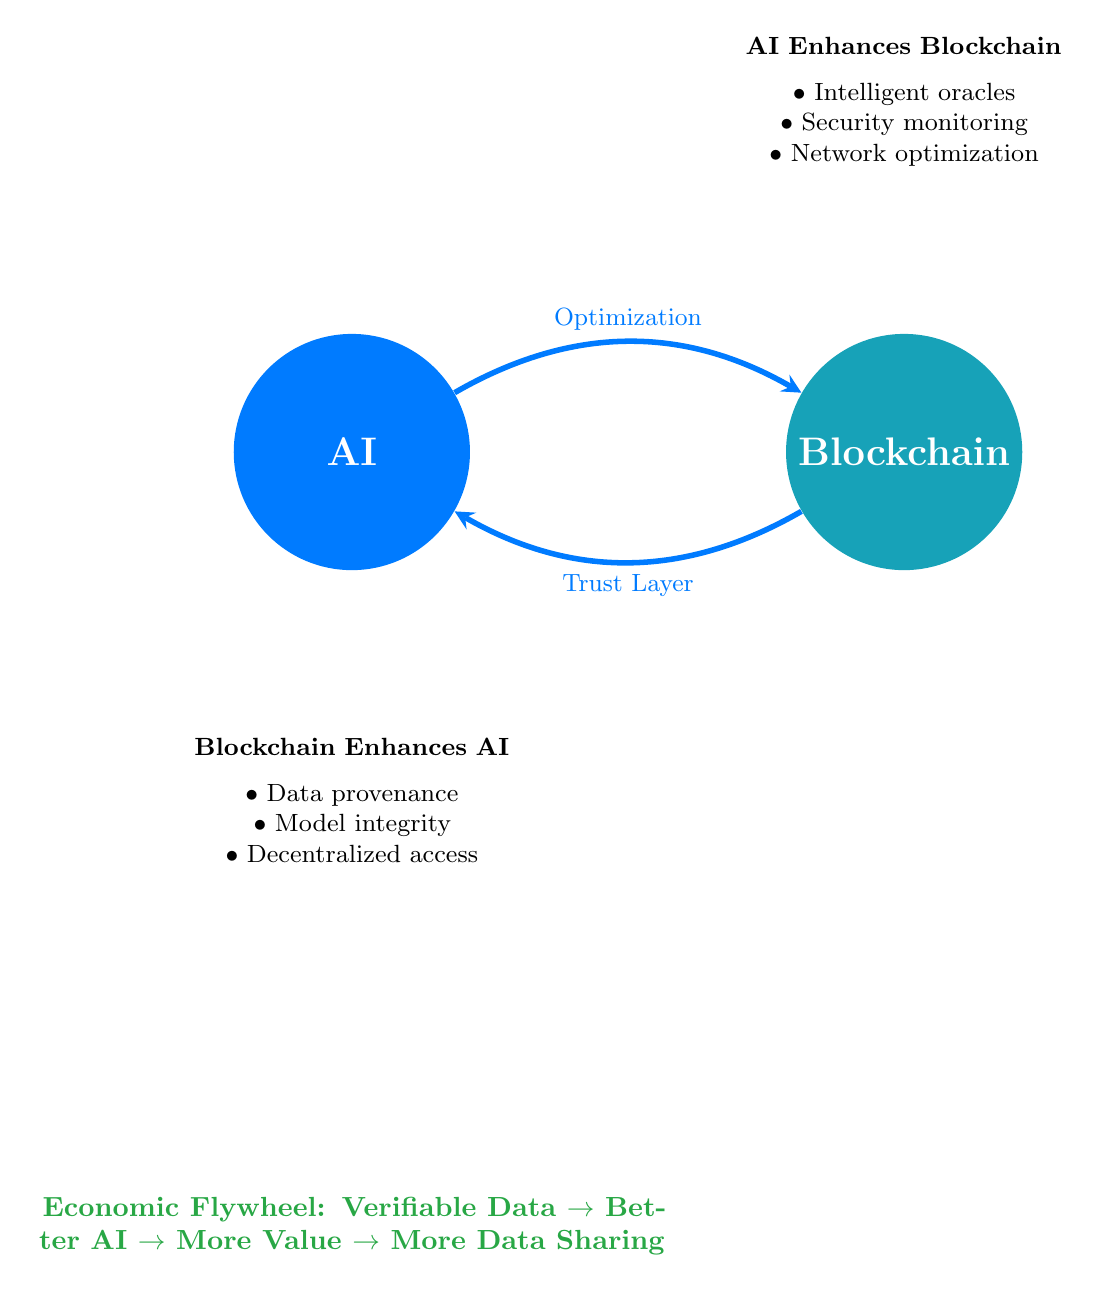
\begin{tikzpicture}[
    node distance=4cm,
    every node/.style={align=center},
    arrow/.style={->,>=stealth,line width=2pt,primaryblue}
]    % Central nodes
    \node[circle, fill=primaryblue, text=white, minimum size=3cm, font=\Large\bfseries] (ai) {AI};
    \node[circle, fill=secondaryblue, text=white, minimum size=3cm, font=\Large\bfseries, right=of ai] (blockchain) {Blockchain};
    
    % AI enhances Blockchain
    \node[above=2cm of blockchain, text width=4cm, font=\small] (ai-enhance) {
        \textbf{AI Enhances Blockchain}\\[0.2cm]
        $\bullet$ Intelligent oracles\\
        $\bullet$ Security monitoring\\
        $\bullet$ Network optimization
    };
    
    % Blockchain enhances AI
    \node[below=2cm of ai, text width=4cm, font=\small] (blockchain-enhance) {
        \textbf{Blockchain Enhances AI}\\[0.2cm]
        $\bullet$ Data provenance\\
        $\bullet$ Model integrity\\
        $\bullet$ Decentralized access
    };
    
    % Arrows
    \draw[arrow, bend left=30] (ai) to node[above, font=\small] {Optimization} (blockchain);
    \draw[arrow, bend left=30] (blockchain) to node[below, font=\small] {Trust Layer} (ai);
    
    % Value creation
    \node[below=of blockchain-enhance, text width=8cm, font=\normalsize\bfseries, text=accentgreen] {
        Economic Flywheel: Verifiable Data $\rightarrow$ Better AI $\rightarrow$ More Value $\rightarrow$ More Data Sharing
    };
\end{tikzpicture}
\caption{The Symbiotic Relationship Between AI and Blockchain}
\end{figure}
\subsection{AI Enhances Blockchain}

AI brings intelligence and optimization to blockchain networks:

\begin{itemize}
    \item \textbf{Intelligent Oracles:} AI algorithms analyze off-chain data feeds to verify accuracy before submission to blockchain oracles
    \item \textbf{Security Enhancement:} AI actively monitors network activity and smart contract code to detect vulnerabilities
    \item \textbf{Predictive Optimization:} AI analyzes historical transaction data to predict and prevent network congestion
\end{itemize}

\subsection{Blockchain Enhances AI}

Conversely, blockchain provides a foundational layer of trust for AI systems:

\begin{keypoint}[Solving the Black Box Problem]
By recording data provenance on an immutable ledger, blockchain creates a verifiable audit trail, showing precisely what data was used to train an AI model. This is critical for developing ethical and regulatory-compliant AI.
\end{keypoint}

\begin{marketfigure}[Key Growth Drivers for Blockchain AI]
\begin{itemize}
    \item \textbf{Healthcare:} Forecast to grow from \$0.93B (2024) to \$18.0B (2035)
    \item \textbf{BFSI:} Expected to exhibit the highest CAGR for security and compliance
    \item \textbf{Cyber Security:} Rising threats drive adoption of integrated AI-blockchain solutions
\end{itemize}
\end{marketfigure}

\section{The Evolving Nature of Digital Value}

The convergence is giving rise to entirely new classes of digital assets that defy traditional categorization:

\begin{enumerate}
    \item \textbf{Self-executing smart contracts} managing complex financial agreements with built-in compliance and automated execution
    \item \textbf{Decentralized ecosystems} governed by their participants through transparent, algorithmic decision-making processes
    \item \textbf{Autonomous AI agents} capable of performing tasks, learning from interactions, and generating revenue independently
\end{enumerate}

These new assets possess unique properties that distinguish them from traditional digital or physical assets. An AI agent is not a finished product; it is a dynamic system that learns and adapts over time. Its value is not fixed but fluid, increasing as it acquires new data, improves its performance, and expands its capabilities.

\begin{keypoint}[Dynamic Value Creation]
Unlike traditional assets whose value is largely determined by scarcity or utility, convergent economy assets create value through continuous learning, adaptation, and network effects. Their worth grows with usage and interaction.
\end{keypoint}

\subsection{Characteristics of Convergent Assets}

The convergence is giving birth to a new category of digital assets that possess unique characteristics:

\begin{itemize}
    \item \textbf{Intelligent Assets}: Digital assets that can learn, adapt, and optimize their own performance based on market conditions and user interactions
    \item \textbf{Autonomous Revenue Generation}: Assets capable of generating income without human intervention through automated trading, service provision, or resource optimization
    \item \textbf{Verifiable Provenance}: Complete audit trails ensuring authenticity, compliance, and transparent ownership history
    \item \textbf{Programmable Governance}: Built-in rules for ownership, usage rights, value distribution, and stakeholder decision-making
    \item \textbf{Composable Functionality}: Assets that can be combined with others to create new value propositions and business models
\end{itemize}

\subsection{Market Implications}

This evolution in digital value creation has profound implications for traditional business models and investment strategies. Companies that can successfully tokenize and monetize their AI capabilities, software assets, and data resources will gain significant competitive advantages in the emerging convergent economy.

% Chapter 3
\chapter{The Trust Revolution: Blockchain as the Foundational Layer}

The ``why'' behind this powerful convergence is rooted in a single, fundamental concept: trust. In an increasingly digital world fraught with data breaches, misinformation, and opaque algorithms, blockchain technology offers a new paradigm for establishing trust.

\section{The Core Tenets of Blockchain Trust}

Blockchain's ability to engender trust is derived from its three core architectural principles:

\begin{figure}[H]
\centering
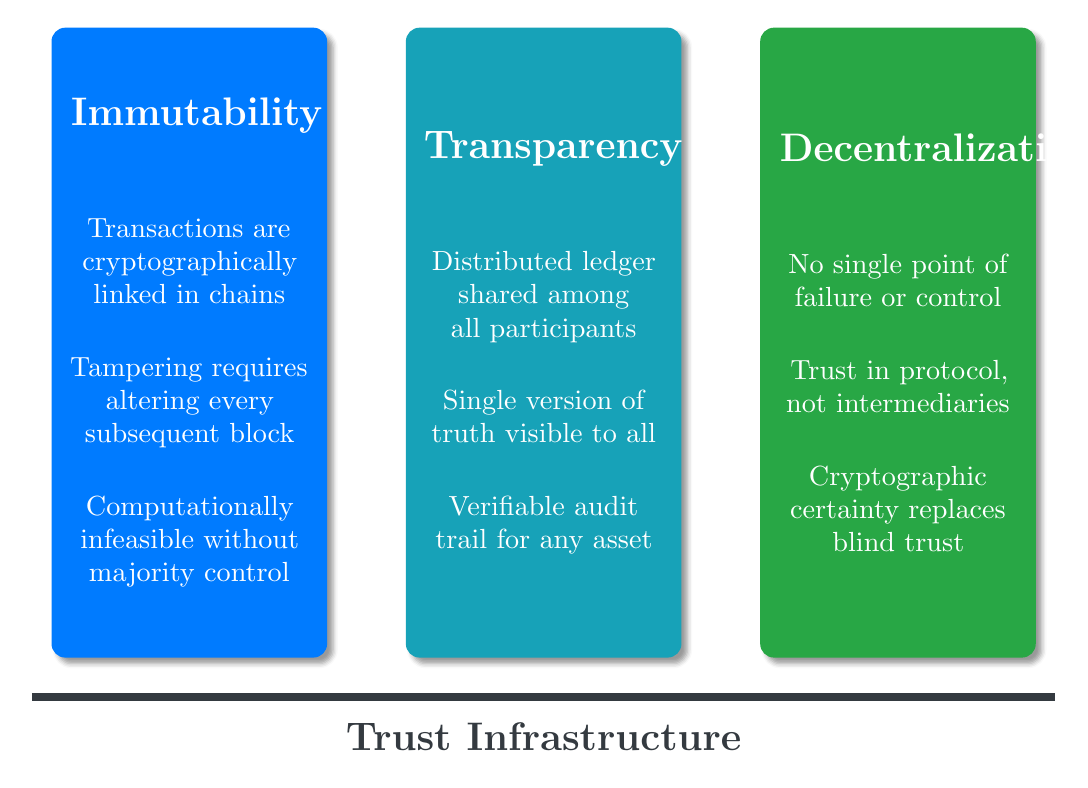
\begin{tikzpicture}[
    pillar/.style={
        rectangle,
        rounded corners=5pt,
        minimum width=3.5cm,
        minimum height=8cm,
        text width=3cm,
        align=center,
        font=\normalsize,
        text=white,
        blur shadow
    }
]
    % Pillars
    \node[pillar, fill=primaryblue] (immut) at (0,0) {
        \textbf{\Large Immutability}\\[1cm]
        Transactions are crypto\-graphically linked in chains\\[0.5cm]
        Tampering requires altering every subsequent block\\[0.5cm]
        Computationally infeasible without majority control
    };    
    \node[pillar, fill=secondaryblue] (trans) at (4.5,0) {
        \textbf{\Large Transparency}\\[1cm]
        Distributed ledger shared among all participants\\[0.5cm]
        Single version of truth visible to all\\[0.5cm]
        Verifiable audit trail for any asset
    };
    
    \node[pillar, fill=accentgreen] (decent) at (9,0) {
        \textbf{\Large Decentralization}\\[1cm]
        No single point of failure or control\\[0.5cm]
        Trust in protocol, not inter\-mediaries\\[0.5cm]
        Crypto\-graphic certainty replaces blind trust
    };
    
    % Foundation
    \draw[line width=3pt, darkgray] (-2,-4.5) -- (11,-4.5);
    \node[font=\Large\bfseries, text=darkgray] at (4.5,-5) {Trust Infrastructure};
\end{tikzpicture}
\caption{The Three Pillars of Blockchain Trust}
\end{figure}

\section{Addressing the AI ``Black Box''}

The trust infrastructure of blockchain directly addresses one of the most significant challenges facing the AI industry: the ``black box'' problem.

\subsection{Verifiable Data Provenance}

By recording data sources and usage rights on-chain, blockchain provides definitive proof of the data used to train an AI model. Stakeholders can verify:
\begin{itemize}
    \item Where the data originated
    \item Who owns it
    \item Whether it was used in accordance with permissioned rights
\end{itemize}

\subsection{Model Integrity and Versioning}

\begin{tcolorbox}[
    colback=lightgray,
    colframe=primaryblue,
    title=Implementation Example,
    fonttitle=\bfseries
]
\begin{verbatim}
// Cryptographic hash of AI model
modelHash = SHA256(model.architecture + model.parameters)

// Record on blockchain
blockchain.record({
    modelHash: modelHash,
    timestamp: Date.now(),
    version: "2.1.0",
    validator: auditor.address
})
\end{verbatim}
\end{tcolorbox}

\section{Securing Intellectual Property in the Age of AI-Generated Code}

The proliferation of AI-powered development tools is introducing unprecedented complexity to the world of intellectual property. With AI assistants now capable of generating 25-30\% of code in some major tech companies, fundamental questions arise:
\begin{keypoint}[Critical Questions]
\begin{itemize}
    \item Who owns the code generated by an AI?
    \item How can a developer prove the originality of a novel algorithm created with AI assistance?
    \item What are the liability implications of AI-generated code?
\end{itemize}
\end{keypoint}

Blockchain offers a powerful mechanism to bring clarity and security to this new landscape through decentralized, immutable, and time-stamped IP registries.

% Chapter 4
\chapter{Tokenization: The Unifying Framework\\for Monetization and Governance}

If blockchain provides the ``why'' for the convergent economy---the foundation of trust---then tokenization provides the ``how.'' It is the technical and economic framework that allows the novel forms of value created at the intersection of AI and software to be defined, owned, governed, and traded.

\section{The Tokenization Market: A Pillar of the Convergent Economy}

The market for tokenization is itself a substantial and rapidly growing sector, reflecting its increasing importance as a foundational technology.

\begin{marketfigure}[Tokenization Market Growth]
\centering
\begin{tabular}{lrr}
\toprule
\textbf{Segment} & \textbf{2025 Size} & \textbf{2030 Forecast} \\
& (USD Billion) & (USD Billion) \\
\midrule
Real Estate Tokenization & \marketvalue{2.4}{} & \marketvalue{18.7}{} \\
Art \& Collectibles & \marketvalue{1.8}{} & \marketvalue{12.3}{} \\
Intellectual Property & \marketvalue{0.9}{} & \marketvalue{8.4}{} \\
Software \& Digital Assets & \marketvalue{0.6}{} & \marketvalue{5.2}{} \\
\bottomrule
\end{tabular}
\end{marketfigure}

\section{The ERC-1155 Advantage: Multi-Token Efficiency}

The ERC-1155 standard represents a breakthrough in token design, enabling a single smart contract to manage multiple token types simultaneously.

\begin{keypoint}[ERC-1155 Technical Advantages]
\begin{itemize}
    \item \textbf{Gas Efficiency}: Batch operations reduce transaction costs by up to 90\%
    \item \textbf{Flexibility}: Single contract manages both fungible and non-fungible tokens
    \item \textbf{Atomic Swaps}: Multiple tokens exchanged in single transaction
    \item \textbf{Rich Metadata}: Dynamic properties and detailed asset descriptions
\end{itemize}
\end{keypoint}

\subsection{Real-World Tokenization Applications}

The convergent economy enables sophisticated tokenization scenarios:

\begin{enumerate}
    \item \textbf{AI Model Licensing}: Different access levels (inference, training, commercial use) as separate token types
    \item \textbf{Software Component Markets}: Individual modules, APIs, and features as tradeable assets
    \item \textbf{Data Rights Management}: Granular permissions for data usage, training, and distribution
    \item \textbf{Decentralized Governance}: Voting rights proportional to contribution and stake
\end{enumerate}

\section{The Economic Flywheel Effect}

Tokenization creates a powerful economic flywheel in the convergent economy:

\vspace{0.5cm}

\begin{center}
\textbf{The Tokenization Economic Flywheel}

\vspace{0.3cm}

\begin{tabular}{c}
\colorbox{ocean}{\textcolor{white}{\textbf{Tokenized Assets}}} \\
$\downarrow$ \\
Increased Liquidity $\rightarrow$ Higher Valuations $\rightarrow$ More Investment \\
$\downarrow$ \\
Greater Innovation $\rightarrow$ More Assets $\rightarrow$ Wider Adoption \\
$\uparrow$ \\
\textit{(Cycle continues, creating a self-reinforcing flywheel effect)}
\end{tabular}
\end{center}

\vspace{0.5cm}

\subsection{Flywheel Mechanics and Market Dynamics}

The tokenization flywheel operates through several interconnected mechanisms that create compounding value:

\begin{enumerate}
    \item \textbf{Liquidity Premium}: Tokenized assets trade 24/7 in global markets, commanding higher valuations than illiquid alternatives
    \item \textbf{Fractional Ownership}: Lower barriers to entry attract broader investor participation
    \item \textbf{Programmable Value}: Smart contracts enable automated revenue distribution and governance
    \item \textbf{Composability}: Tokenized assets can be combined into new financial products and services
\end{enumerate}

\begin{keypoint}[Network Effects]
As more assets become tokenized, the infrastructure becomes more valuable, attracting additional participants and creating a self-reinforcing cycle of adoption and innovation.
\end{keypoint}

This flywheel effect is particularly pronounced in the convergent economy, where AI-enhanced blockchain systems can automatically optimize tokenization strategies, predict market demand, and execute complex multi-asset transactions.

% Chapter 5
\chapter{Market Opportunities: Where to Invest and Build}

The convergent economy presents significant opportunities across multiple market segments. Analysis reveals that the most promising near-term opportunities lie in horizontal, enabling infrastructure that supports the broader ecosystem.

\section{Tokenization-as-a-Service (TaaS) Platforms}

TaaS platforms represent the most immediate and scalable opportunity, providing comprehensive infrastructure for digital asset tokenization.

\subsection{Market Sizing and Opportunity}

\begin{marketfigure}[TaaS Market Opportunity]
\begin{itemize}
    \item \textbf{Addressable Market}: \marketvalue{50+ billion}{} in tokenizable assets by 2030
    \item \textbf{Platform Revenue}: 2-5\% transaction fees plus subscription models
    \item \textbf{Growth Drivers}: Enterprise adoption, regulatory clarity, improved UX
    \item \textbf{Key Players}: Emerging market with no dominant leaders yet
\end{itemize}
\end{marketfigure}

\subsection{TaaS Value Proposition}

\begin{itemize}
    \item \textbf{Technical Infrastructure}: Complete blockchain deployment and smart contract management
    \item \textbf{Regulatory Compliance}: Built-in frameworks for securities law compliance
    \item \textbf{User Experience}: Simplified interfaces abstracting blockchain complexity
    \item \textbf{Integration Services}: APIs and SDKs for existing enterprise systems
    \item \textbf{White-Label Solutions}: Customizable branding and user experiences
\end{itemize}

\section{Digital Asset Marketplaces}

White-label marketplace infrastructure enables rapid deployment of specialized trading platforms for the convergent economy.

\begin{enumerate}
    \item \textbf{AI Model Marketplaces}: Platforms for trading pre-trained models, datasets, and inference services
    \item \textbf{Software Component Exchanges}: Marketplaces for reusable code modules, APIs, and development tools
    \item \textbf{IP Licensing Platforms}: Automated licensing and royalty distribution for intellectual property
    \item \textbf{Governance Token Exchanges}: Specialized trading venues for DAO and protocol governance tokens
\end{enumerate}

\section{Smart Contract Auditing and Security Services}

As the ecosystem matures and handles higher-value assets, security becomes paramount.

\begin{keypoint}[Security Market Drivers]
\begin{itemize}
    \item \textbf{High-Value Assets}: Tokenized assets worth millions require robust security
    \item \textbf{Regulatory Requirements}: Compliance mandates for financial applications
    \item \textbf{Insurance Integration}: Risk assessment for digital asset coverage
    \item \textbf{Continuous Monitoring}: Ongoing surveillance of deployed contracts
\end{itemize}
\end{keypoint}

\subsection{Service Categories}

\begin{itemize}
    \item \textbf{Automated Code Analysis}: AI-powered vulnerability detection and analysis
    \item \textbf{Formal Verification}: Mathematical proof of smart contract correctness
    \item \textbf{Penetration Testing}: Simulated attacks to identify security weaknesses
    \item \textbf{Compliance Auditing}: Verification of regulatory requirement adherence
\end{itemize}

% Chapter 6
\chapter{Challenges and Risk Factors}

While the convergent economy presents significant opportunities, several challenges must be addressed for mainstream adoption.

\section{Regulatory Uncertainty: The Primary Headwind}

Regulatory uncertainty remains the most significant challenge facing the convergent economy.

\begin{figure}[H]
\centering
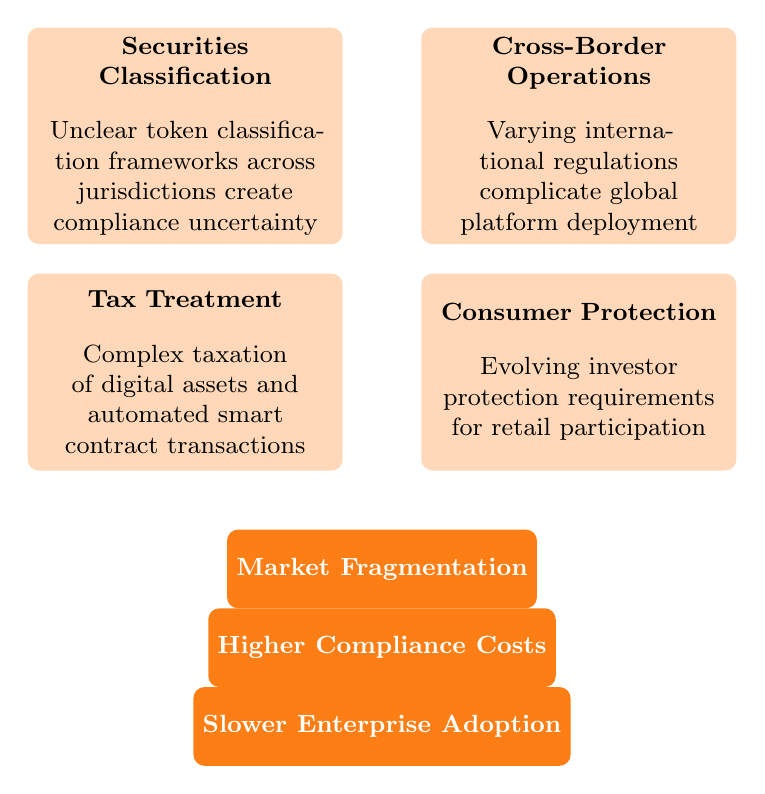
\begin{tikzpicture}[
    challenge/.style={rectangle, rounded corners, fill=warnorange!30, minimum width=4cm, minimum height=2.5cm, text width=3.5cm, align=center, font=\small},
    impact/.style={rectangle, rounded corners, fill=warnorange, text=white, minimum width=3cm, minimum height=1cm, font=\small\bfseries, text centered}
]
    \node[challenge] (securities) at (0,3) {
        \textbf{Securities Classification}\\[0.3cm]
        Unclear token classification frameworks across jurisdictions create compliance uncertainty
    };
    
    \node[challenge] (cross) at (5,3) {
        \textbf{Cross-Border Operations}\\[0.3cm]
        Varying international regulations complicate global platform deployment
    };
    
    \node[challenge] (tax) at (0,0) {
        \textbf{Tax Treatment}\\[0.3cm]
        Complex taxation of digital assets and automated smart contract transactions
    };
    
    \node[challenge] (consumer) at (5,0) {
        \textbf{Consumer Protection}\\[0.3cm]
        Evolving investor protection requirements for retail participation
    };
    
    % Impact arrows and labels
    \node[impact] at (2.5,-2.5) {Market Fragmentation};
    \node[impact] at (2.5,-3.5) {Higher Compliance Costs};
    \node[impact] at (2.5,-4.5) {Slower Enterprise Adoption};
\end{tikzpicture}
\caption{Regulatory Challenges and Market Impact}
\end{figure}

\section{Technical and Scalability Challenges}

\begin{itemize}
    \item \textbf{Blockchain Throughput}: Current limitations (15-7,000 TPS) vs. traditional systems (65,000+ TPS)
    \item \textbf{Cross-Chain Interoperability}: Immature protocols for multi-blockchain applications
    \item \textbf{User Experience Complexity}: Technical barriers preventing mainstream adoption
    \item \textbf{Energy Consumption}: Environmental sustainability concerns for some blockchain networks
\end{itemize}

\section{Market and Adoption Risks}

\begin{enumerate}
    \item \textbf{Price Volatility}: High volatility affecting business planning and user adoption
    \item \textbf{Liquidity Constraints}: Thin markets for specialized digital assets
    \item \textbf{Security Vulnerabilities}: Smart contract bugs and hacking incidents
    \item \textbf{Slower Than Expected Adoption}: Enterprise and consumer uptake may lag projections
\end{enumerate}

% Chapter 7
\chapter{Strategic Outlook and Conclusions}

The convergence of AI, software development, and blockchain technology, unified by tokenization, represents a fundamental shift toward a more transparent, efficient, and liquid global digital economy.

\section{Key Market Insights}

\begin{keypoint}[Executive Summary]
\begin{itemize}
    \item Combined market opportunity exceeds \marketvalue{5 trillion}{} by 2034
    \item Blockchain AI demonstrates premium growth at \cagr{37.18}, indicating significant value-add
    \item Tokenization enables revolutionary models of digital asset ownership and monetization
    \item Near-term opportunities concentrated in enabling infrastructure and services
    \item Regulatory clarity will be the key catalyst for mainstream enterprise adoption
\end{itemize}
\end{keypoint}

\section{Strategic Recommendations}

\subsection{For Investors}
\begin{itemize}
    \item \textbf{Focus on Infrastructure}: Prioritize horizontal platforms (TaaS, marketplaces, security)
    \item \textbf{Diversify Across Stack}: Balance investments across AI, blockchain, and software layers
    \item \textbf{Monitor Regulatory Developments}: Track policy changes that could accelerate or hinder adoption
    \item \textbf{Consider Timing}: Early infrastructure investments may capture disproportionate value
\end{itemize}

\subsection{For Enterprises}
\begin{itemize}
    \item \textbf{Start with Pilots}: Begin with low-risk proof-of-concept projects
    \item \textbf{Partner Strategically}: Leverage TaaS providers to reduce technical and regulatory risk
    \item \textbf{Build Internal Expertise}: Develop blockchain and tokenization capabilities
    \item \textbf{Prepare for Compliance}: Establish frameworks for regulatory adherence
\end{itemize}

\subsection{For Entrepreneurs}
\begin{itemize}
    \item \textbf{Target Specific Verticals}: Focus on industries with clear tokenization value propositions
    \item \textbf{Build on Standards}: Leverage established protocols (ERC-1155, etc.) for interoperability
    \item \textbf{Prioritize User Experience}: Abstract complexity to enable mainstream adoption
    \item \textbf{Consider B2B2C Models}: White-label solutions may offer faster market entry
\end{itemize}

\section{The Path Forward}

The convergent economy is not a distant future---it is emerging today. The trajectory is clear, driven by powerful economic forces and technological capabilities that are already demonstrable.

\begin{figure}[H]
\centering
\begin{tikzpicture}[
    timeline/.style={->, >=stealth, line width=3pt, primaryblue},
    phase/.style={rectangle, rounded corners, fill=lightgray, minimum width=3.5cm, minimum height=2.5cm, text width=3cm, align=center, font=\small}
]
    % Timeline
    \draw[timeline] (0,0) -- (13,0);
    
    % Phases
    \node[phase, fill=primaryblue!30] at (2.5,2.5) {
        \textbf{2025-2027}\\[0.3cm]
        \textbf{Infrastructure Building}\\[0.2cm]
        • TaaS platforms launch\\[0.1cm]
        • Regulatory frameworks emerge\\[0.1cm]
        • Early enterprise pilots
    };
    
    \node[phase, fill=secondaryblue!30] at (6.5,2.5) {
        \textbf{2028-2030}\\[0.3cm]
        \textbf{Enterprise Adoption}\\[0.2cm]
        • Mainstream business integration\\[0.1cm]
        • Mature security standards\\[0.1cm]
        • Cross-chain interoperability
    };
    
    \node[phase, fill=accentgreen!30] at (10.5,2.5) {
        \textbf{2031+}\\[0.3cm]
        \textbf{Mainstream Integration}\\[0.2cm]
        • Consumer-grade UX\\[0.1cm]
        • Global regulatory harmony\\[0.1cm]
        • Trillion-dollar markets
    };
    
    % Milestones
    \node[below, font=\small] at (2.5,-0.5) {Platform Launch};
    \node[below, font=\small] at (6.5,-0.5) {Enterprise Scale};
    \node[below, font=\small] at (10.5,-0.5) {Mass Adoption};
    
    % Timeline labels
    \node[below, font=\bfseries] at (0,-1.2) {2025};
    \node[below, font=\bfseries] at (13,-1.2) {2035};
\end{tikzpicture}
\caption{Convergent Economy Adoption Timeline}
\end{figure}

\section{Final Thoughts}

The organizations and investors who recognize and act upon this convergence today will be positioned to capture disproportionate value as the convergent economy matures. The future belongs to those who can navigate the intersection of intelligence, decentralization, and tokenized value creation.

The question is not whether this transformation will occur, but how quickly and who will lead it. The convergent economy represents the next chapter in the digital revolution---one where artificial intelligence, software innovation, and blockchain infrastructure combine to create unprecedented opportunities for value creation and exchange.

The time to act is now.

\appendix
\chapter{Market Data Sources and Methodology}

\section{Primary Data Sources}
This analysis draws from multiple authoritative market research sources:

\begin{itemize}
    \item \textbf{Precedence Research} - Global AI Market Analysis and Long-term Projections
    \item \textbf{Grand View Research} - Technology Market Forecasts and Industry Trends
    \item \textbf{Fortune Business Insights} - Blockchain Technology Market Data and Analysis
    \item \textbf{Research and Markets} - Blockchain AI Convergence Market Projections
    \item \textbf{McKinsey Global Institute} - AI Economic Impact Studies and Enterprise Surveys
    \item \textbf{Market Research Future} - Emerging Technology Convergence Analysis
\end{itemize}

\section{Analytical Methodology}

\subsection{Market Sizing Approach}
Market projections utilize compound annual growth rate (CAGR) calculations based on:
\begin{itemize}
    \item Historical market performance data (2020-2024)
    \item Forward-looking industry analysis and expert forecasts
    \item Technology adoption curve modeling
    \item Patent filing trends and R\&D investment flows
    \item Venture capital and private equity investment analysis
\end{itemize}

\subsection{Convergence Opportunity Assessment}
The convergence analysis employs:
\begin{itemize}
    \item Cross-market correlation and synergy analysis
    \item Value chain integration mapping
    \item Technology readiness level assessment
    \item Regulatory impact modeling
    \item Competitive landscape analysis
\end{itemize}

\section{Limitations and Key Assumptions}

\begin{itemize}
    \item Market projections assume continued technological advancement at current pace
    \item Regulatory environment assumed to become more favorable over the projection period
    \item Economic conditions assumed to remain conducive to technology investment
    \item All monetary figures presented in USD unless otherwise specified
    \item Projections subject to revision based on regulatory developments and market conditions
\end{itemize}

\section{About the Analysis}

This report represents an independent analysis of publicly available market data and industry trends. Projections are based on current market conditions and may be subject to significant variation based on regulatory, technological, and economic developments.

\end{document}darkgray}
]
% Conservative projection
\addplot[
    color=primaryblue,
    line width=2pt,
    mark=square*,
    mark options={scale=1.5}
] coordinates {
    (2025,0.00413)
    (2026,0.00523)
    (2027,0.00663)
    (2028,0.00840)
    (2029,0.01065)
};
\addlegendentry{Conservative Estimate (Billions)}

% BCG projection
\addplot[
    color=accentgreen,
    line width=3pt,
    mark=triangle*,
    mark options={scale=2},
    dashed
] coordinates {
    (2025,2.5)
    (2026,4.8)
    (2027,7.3)
    (2028,10.2)
    (2029,13.1)
    (2030,16.1)
};
\addlegendentry{BCG Projection (Trillions)}
\end{axis}
\end{tikzpicture}
\caption{Tokenization Market Projections: From Billions to Trillions}
\end{figure}
\begin{keypoint}[Transformative Potential]
Boston Consulting Group estimates that the value of tokenized assets could reach \marketvalue{16.1 trillion}{} by 2030, representing 10\% of global GDP.
\end{keypoint}

At its core, tokenization is the process of converting the rights associated with an asset into a digital token that resides on a blockchain. This digital representation unlocks several powerful economic benefits:

\begin{itemize}
    \item \textbf{Fractional ownership}: High-value assets divided into accessible units
    \item \textbf{Enhanced liquidity}: For traditionally illiquid asset classes
    \item \textbf{Democratized access}: Broader base of investors and participants
\end{itemize}

\section{Technical Foundation: The ERC-1155 Multi-Token Standard}

The evolution of token standards has been crucial to enabling complex tokenization use cases.

\begin{figure}[H]
\centering
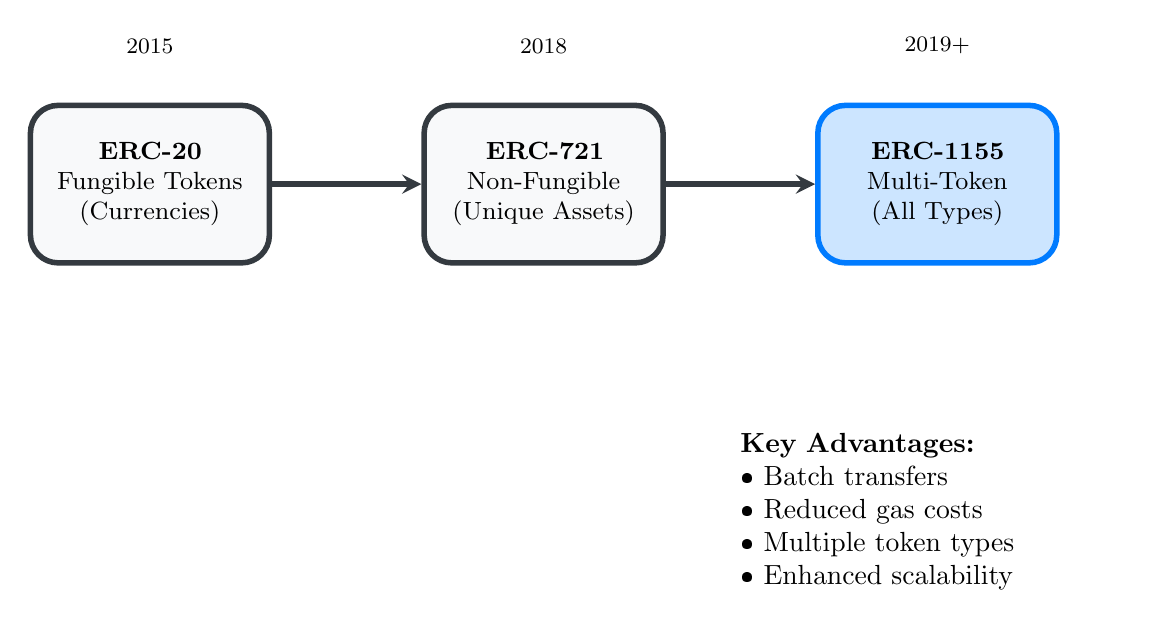
\begin{tikzpicture}[
    token/.style={
        rectangle,
        rounded corners=10pt,
        minimum width=3cm,
        minimum height=2cm,
        text width=2.8cm,
        align=center,
        font=\small,
        draw,
        line width=2pt
    },
    arrow/.style={->,>=stealth,line width=2pt,darkgray}
]    % Token evolution
    \node[token, fill=lightgray, draw=darkgray] (erc20) at (0,0) {
        \textbf{ERC-20}\\
        Fungible Tokens\\
        (Currencies)
    };
    
    \node[token, fill=lightgray, draw=darkgray] (erc721) at (5,0) {
        \textbf{ERC-721}\\
        Non-Fungible\\
        (Unique Assets)
    };
    
    \node[token, fill=primaryblue!20, draw=primaryblue] (erc1155) at (10,0) {
        \textbf{ERC-1155}\\
        Multi-Token\\
        (All Types)
    };
    
    % Arrows
    \draw[arrow] (erc20) -- (erc721);
    \draw[arrow] (erc721) -- (erc1155);
    
    % Labels
    \node[above=0.5cm of erc20, font=\footnotesize] {2015};
    \node[above=0.5cm of erc721, font=\footnotesize] {2018};
    \node[above=0.5cm of erc1155, font=\footnotesize] {2019+};
    
    % Benefits box
    \node[below=2cm of erc1155, text width=5cm, align=left] {
        \textbf{Key Advantages:}\\
        • Batch transfers\\
        • Reduced gas costs\\
        • Multiple token types\\
        • Enhanced scalability
    };
\end{tikzpicture}
\caption{Evolution of Ethereum Token Standards}
\end{figure}
\subsection{ERC-1155: The Swiss Army Knife of Tokenization}

The ERC-1155 standard allows a single smart contract to mint, manage, and transfer multiple different token types simultaneously. Consider an AI-powered software project using ERC-1155:

\begin{marketfigure}[Unified Token Architecture]
\begin{itemize}
    \item \textbf{Fungible utility tokens}: API access on pay-per-call basis
    \item \textbf{Non-fungible token (NFT)}: Legal ownership of underlying IP
    \item \textbf{Semi-fungible governance tokens}: Voting rights for community members
\end{itemize}
All managed within a single, efficient smart contract
\end{marketfigure}

\section{Monetizing the Unmonetizable: New Business Models}

Tokenization unlocks a plethora of new business models that were previously impossible:

\subsection{Tokenizing AI Agents}

\begin{tcolorbox}[
    enhanced,
    colback=primaryblue!5,
    colframe=primaryblue,
    title=AI Agent Token Model,
    fonttitle=\bfseries,
    drop fuzzy shadow
]
\begin{enumerate}
    \item \textbf{Development Funding}: Sell tokens to fund AI model creation
    \item \textbf{Access Rights}: Tokens grant API access to agent's capabilities
    \item \textbf{Revenue Sharing}: Token holders receive share of generated revenue
    \item \textbf{Governance}: Vote on agent's development priorities
    \item \textbf{Value Appreciation}: Token price reflects agent's improving performance
\end{enumerate}
\end{tcolorbox}
\subsection{Tokenizing Software Modules \& IP}

This model fundamentally changes the economics of software creation:

\begin{table}[H]
\centering
\caption{Token Types for Software IP}
\begin{tabular}{p{3cm}p{9cm}}
\toprule
\textbf{Token Type} & \textbf{Rights \& Benefits} \\
\midrule
\textcolor{accentgreen}{\textbf{Royalty Tokens}} & Holders receive percentage of future revenue generated by the software \\
\textcolor{primaryblue}{\textbf{Equity Tokens}} & Represent fractional ownership of the IP itself \\
\textcolor{secondaryblue}{\textbf{Utility Tokens}} & Grant the right to use the software or access specific features \\
\bottomrule
\end{tabular}
\end{table}

\subsection{Automated Royalties via Smart Contracts}

\begin{figure}[H]
\centering
\begin{tikzpicture}[
    box/.style={
        rectangle,
        rounded corners=5pt,
        minimum width=3cm,
        minimum height=1.5cm,
        align=center,
        font=\small
    },
    arrow/.style={->,>=stealth,line width=1.5pt}
]    % Flow diagram
    \node[box, fill=lightgray, draw=darkgray] (usage) at (0,0) {Usage Event\\(API call, resale)};
    \node[box, fill=primaryblue!20, draw=primaryblue] (smart) at (5,0) {Smart Contract\\Executes};
    \node[box, fill=accentgreen!20, draw=accentgreen] (payment) at (10,0) {Automatic\\Payment};
    
    \draw[arrow] (usage) -- (smart);
    \draw[arrow] (smart) -- (payment);
    
    % Labels
    \node[below=0.5cm of smart, text width=5cm, align=center, font=\footnotesize] {
        Transparent • Instantaneous • No intermediaries
    };
\end{tikzpicture}
\caption{Automated Royalty Distribution Flow}
\end{figure}

\section{The New Digital Bazaars: Marketplaces for Tokenized Assets}

A vibrant ecosystem of specialized marketplaces is emerging to facilitate the exchange of tokenized assets:

\begin{table}[H]
\centering
\caption{Leading Tokenization Platforms and Marketplaces}
\begin{tabularx}{\textwidth}{lXl}
\toprule
\textbf{Platform} & \textbf{Focus Area} & \textbf{Key Feature} \\
\midrule
Tokeny & Security tokens, regulatory compliance & End-to-end infrastructure \\
Securitize & Digital securities & Institutional-grade custody \\
Polymath & Security token creation & Regulatory automation \\
TokenFi & AI-powered tokenization & Natural language interface \\
Akash Network & Decentralized compute & GPU marketplace \\
\bottomrule
\end{tabularx}
\end{table}
\subsection{Tokenization Use Cases at the Convergence}

\begin{longtable}{p{3cm}p{3cm}p{2.5cm}p{4cm}}
\caption{Real-World Tokenization Applications} \\
\toprule
\textbf{Use Case} & \textbf{Asset Tokenized} & \textbf{Token Types} & \textbf{Monetization} \\
\midrule
\endfirsthead

\multicolumn{4}{c}{\tablename\ \thetable\ -- \textit{Continued from previous page}} \\
\toprule
\textbf{Use Case} & \textbf{Asset Tokenized} & \textbf{Token Types} & \textbf{Monetization} \\
\midrule
\endhead

\midrule
\multicolumn{4}{r}{\textit{Continued on next page}} \\
\endfoot

\bottomrule
\endlastfoot

AI Model Monetization & Trained ML model & Utility, Royalty & Pay-per-API-call; revenue sharing \\
Fractional Software Licensing & Software licenses & Equity, Utility & Sale of ownership tokens; access rights \\
Automated IP Royalties & AI-generated art/music & Royalty NFT & Smart contract distributes secondary sale proceeds \\
Decentralized Compute & GPU processing power & Utility & Token payment for compute resources \\
Token-Governed AI & Open-source AI project & Governance & Voting on technical roadmap and treasury \\
\end{longtable}
% Chapter 5
\chapter{The Evolving Developer: AI's Transformation of Software Creation and Value}

The technological shifts driven by AI are profoundly reshaping the very nature of software development and the role of the developer. As AI changes \textit{what} developers create, tokenization provides the framework for how that new form of value is owned and monetized.

\section{From Coder to Conductor: How AI is Reshaping the Developer Role}

\begin{figure}[H]
\centering
\begin{tikzpicture}[
    role/.style={
        rectangle,
        rounded corners=10pt,
        minimum width=4cm,
        minimum height=3cm,
        text width=3.5cm,
        align=center,
        font=\normalsize,
        draw,
        line width=2pt
    },
    arrow/.style={->,>=stealth,line width=3pt,primaryblue}
]
    % Traditional role
    \node[role, fill=lightgray, draw=darkgray] (traditional) at (0,0) {
        \textbf{Traditional Developer}\\[0.3cm]
        • Manual coding\\
        • Line-by-line authorship\\
        • Syntax focus
    };    
    % New role
    \node[role, fill=primaryblue!20, draw=primaryblue] (modern) at (8,0) {
        \textbf{AI-Era Developer}\\[0.3cm]
        • System architect\\
        • AI conductor\\
        • Problem framer
    };
    
    % Arrow with label
    \draw[arrow] (traditional) -- node[above, font=\small\bfseries] {AI Integration} (modern);
    
    % Statistics
    \node[below=1.5cm of traditional, text width=4cm, align=center] {
        \textbf{2022}\\
        AI generates 2\% of code
    };
    
    \node[below=1.5cm of modern, text width=4cm, align=center] {
        \textbf{2024}\\
        AI generates 25-30\% of code\\
        \textcolor{accentgreen}{55\% faster development}
    };
\end{tikzpicture}
\caption{The Evolution of the Developer Role}
\end{figure}

\subsection{The New Core Competencies}

The most valuable activities are no longer line-by-line code writing, but rather:

\begin{keypoint}[Critical Skills for AI-Era Development]
\begin{enumerate}
    \item \textbf{Problem Framing}: Articulating intentions and requirements to AI systems
    \item \textbf{Code Curation}: Assessing machine-generated logic for quality and security
    \item \textbf{Strategic Decision-Making}: Making nuanced trade-offs AI cannot handle
    \item \textbf{System Integration}: Managing the crucial final 30\% requiring human expertise
\end{enumerate}
\end{keypoint}
\section{Defining the New ``Output'': Why AI-Generated Assets are Ripe for Tokenization}

The product of AI-assisted development is often not static software, but dynamic and intelligent assets:

\begin{marketfigure}[The Monetization Gap]
\textbf{Traditional Model}: Static software → Fixed license → One-time payment\\[0.3cm]
\textbf{New Reality}: Dynamic AI agent → Continuous learning → Increasing value\\[0.3cm]
\textbf{Solution}: Tokenization → Real-time value capture → Liquid markets
\end{marketfigure}

\subsection{The Open-Source Revolution}

Tokenization transforms open-source collaboration from altruistic endeavor to viable economic engine:

\begin{figure}[H]
\centering
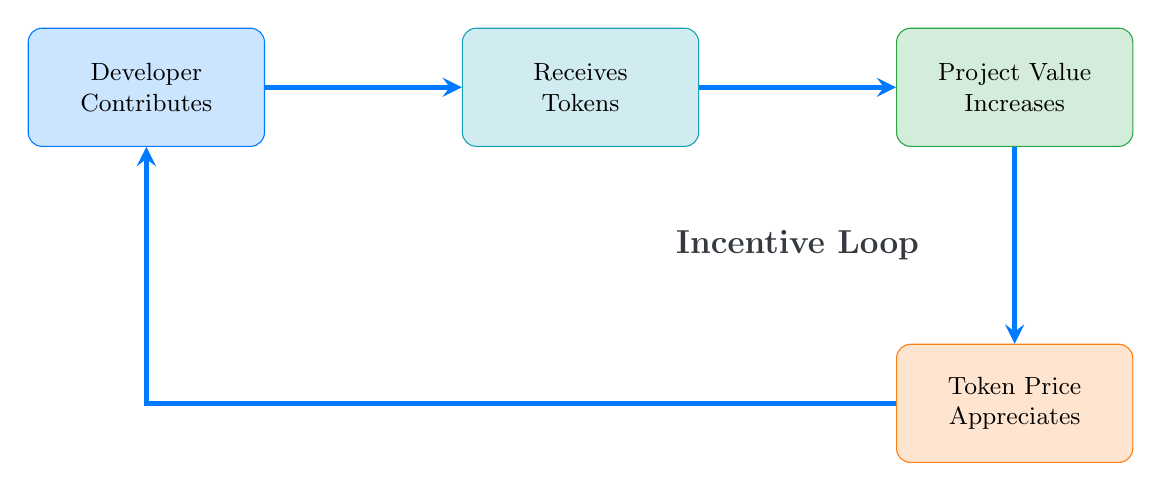
\begin{tikzpicture}[
    node distance=2.5cm,
    process/.style={
        rectangle,
        rounded corners=5pt,
        minimum width=3cm,
        minimum height=1.5cm,
        align=center,
        font=\small
    },
    arrow/.style={->,>=stealth,line width=2pt,primaryblue}
]
    % Process flow
    \node[process, fill=primaryblue!20, draw=primaryblue] (contribute) {Developer\\Contributes};
    \node[process, fill=secondaryblue!20, draw=secondaryblue, right=of contribute] (reward) {Receives\\Tokens};
    \node[process, fill=accentgreen!20, draw=accentgreen, right=of reward] (value) {Project Value\\Increases};
    \node[process, fill=warnorange!20, draw=warnorange, below=of value] (price) {Token Price\\Appreciates};    
    % Arrows
    \draw[arrow] (contribute) -- (reward);
    \draw[arrow] (reward) -- (value);
    \draw[arrow] (value) -- (price);
    \draw[arrow] (price) -| (contribute);
    
    % Center label
    \node[font=\large\bfseries, text=darkgray] at ($(reward)!0.5!(price)$) {Incentive Loop};
\end{tikzpicture}
\caption{Token-Driven Open Source Development Cycle}
\end{figure}

% Chapter 6
\chapter{Strategic Outlook and Recommendations}

The convergence of AI, software development, and blockchain, unified by the economic framework of tokenization, represents one of the most significant investment and strategic opportunities of the next decade.

\section{Investment Thesis: Identifying High-Growth Opportunities}

\subsection{Horizontal Platforms: The ``Picks and Shovels''}

The most significant near-term opportunity lies in building foundational infrastructure:

\begin{tcolorbox}[
    enhanced,
    colback=white,
    colframe=primaryblue,
    title={\textcolor{white}{Investment Priority: Infrastructure Plays}},
    coltitle=white,
    fonttitle=\bfseries\large,
    colbacktitle=primaryblue,
    drop fuzzy shadow
]\begin{enumerate}
    \item \textbf{Tokenization-as-a-Service (TaaS) Platforms}
    \begin{itemize}
        \item Abstract blockchain complexity for enterprises
        \item Managed services for token creation, custody, compliance
        \item The ``AWS for the tokenized economy''
    \end{itemize}
    
    \item \textbf{White-Label Marketplace Solutions}
    \begin{itemize}
        \item Technology for branded digital asset marketplaces
        \item Regulatory compliance built-in
        \item High demand across industries
    \end{itemize}
    
    \item \textbf{Smart Contract Auditing and Security}
    \begin{itemize}
        \item AI-enhanced security auditing
        \item Mission-critical as value locked increases
        \item Non-discretionary expense for serious projects
    \end{itemize}
\end{enumerate}
\end{tcolorbox}

\subsection{Vertical-Specific Marketplaces}

As infrastructure matures, specialized marketplaces will flourish:

\begin{table}[H]
\centering
\caption{High-Potential Vertical Marketplaces}
\begin{tabularx}{\textwidth}{lXc}
\toprule
\textbf{Marketplace Type} & \textbf{Value Proposition} & \textbf{TAM by 2030} \\
\midrule
AI Models and Agents & Trade and license proprietary AI assets & \$50B+ \\
Tokenized Software IP & Fractional licensing of code modules & \$30B+ \\
Decentralized Compute & Open market for GPU resources & \$20B+ \\
\bottomrule
\end{tabularx}
\end{table}
\section{Competitive Landscape: Key Players and Emerging Disruptors}

\begin{figure}[H]
\centering
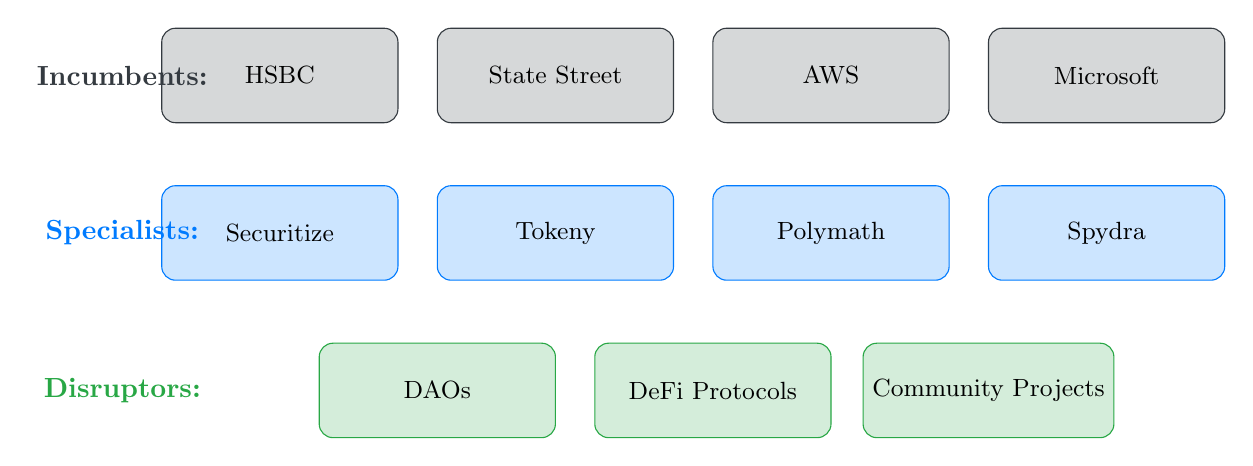
\begin{tikzpicture}[
    company/.style={
        rectangle,
        rounded corners=5pt,
        minimum width=3cm,
        minimum height=1.2cm,
        align=center,
        font=\small
    }
]
    % Incumbents
    \node[company, fill=darkgray!20, draw=darkgray] (hsbc) at (0,0) {HSBC};
    \node[company, fill=darkgray!20, draw=darkgray] (state) at (3.5,0) {State Street};
    \node[company, fill=darkgray!20, draw=darkgray] (aws) at (7,0) {AWS};
    \node[company, fill=darkgray!20, draw=darkgray] (msft) at (10.5,0) {Microsoft};
    
    % Specialists
    \node[company, fill=primaryblue!20, draw=primaryblue] (secure) at (0,-2) {Securitize};
    \node[company, fill=primaryblue!20, draw=primaryblue] (tokeny) at (3.5,-2) {Tokeny};
    \node[company, fill=primaryblue!20, draw=primaryblue] (poly) at (7,-2) {Polymath};
    \node[company, fill=primaryblue!20, draw=primaryblue] (spydra) at (10.5,-2) {Spydra};
    
    % Disruptors
    \node[company, fill=accentgreen!20, draw=accentgreen] (dao1) at (2,-4) {DAOs};
    \node[company, fill=accentgreen!20, draw=accentgreen] (defi) at (5.5,-4) {DeFi Protocols};
    \node[company, fill=accentgreen!20, draw=accentgreen] (comm) at (9,-4) {Community Projects};    
    % Labels
    \node[font=\bfseries, text=darkgray] at (-2,0) {Incumbents:};
    \node[font=\bfseries, text=primaryblue] at (-2,-2) {Specialists:};
    \node[font=\bfseries, text=accentgreen] at (-2,-4) {Disruptors:};
\end{tikzpicture}
\caption{Competitive Landscape Overview}
\end{figure}

\section{Risk Analysis: Navigating the Headwinds}

\begin{table}[H]
\centering
\caption{Key Risk Factors and Mitigation Strategies}
\begin{tabularx}{\textwidth}{p{3cm}Xp{4cm}}
\toprule
\textbf{Risk Category} & \textbf{Description} & \textbf{Mitigation Strategy} \\
\midrule
Regulatory Uncertainty & Ambiguous token classification varies by jurisdiction & Multi-jurisdictional compliance frameworks; proactive regulator engagement \\
Technical Complexity & Smart contract vulnerabilities; developer shortage & Rigorous auditing protocols; investment in developer education \\
Market Adoption & Low initial liquidity for niche assets & Focus on high-demand verticals; strategic partnerships \\
\bottomrule
\end{tabularx}
\end{table}

\section{Concluding Remarks: The Path Forward}

\begin{keypoint}[The Trillion-Dollar Opportunity]
The convergence of AI, software, and blockchain is not an incremental evolution; it is a fundamental re-architecting of how digital value is created, owned, and exchanged. Tokenization stands at the heart of this transformation.
\end{keypoint}
The journey ahead will be complex, but the economic forces driving this shift are undeniable. The destination is a more transparent, efficient, and accessible global economy for digital assets—a paradigm shift that will define the next generation of technology and finance.

\begin{figure}[H]
\centering
\begin{tikzpicture}[
    timeline/.style={
        rectangle,
        rounded corners=5pt,
        minimum width=2.5cm,
        minimum height=1cm,
        align=center,
        font=\footnotesize
    },
    arrow/.style={->,>=stealth,line width=2pt,darkgray}
]
    % Timeline
    \node[timeline, fill=lightgray, draw=darkgray] (now) at (0,0) {2025\\Foundation};
    \node[timeline, fill=primaryblue!20, draw=primaryblue] (near) at (4,0) {2027\\Adoption};
    \node[timeline, fill=secondaryblue!20, draw=secondaryblue] (mid) at (8,0) {2030\\Integration};
    \node[timeline, fill=accentgreen!20, draw=accentgreen] (future) at (12,0) {2034\\Maturity};
    
    % Arrows
    \draw[arrow] (now) -- (near);
    \draw[arrow] (near) -- (mid);
    \draw[arrow] (mid) -- (future);
    
    % Labels
    \node[below=0.5cm of now, text width=2.5cm, align=center, font=\tiny] {Infrastructure\\Building};
    \node[below=0.5cm of near, text width=2.5cm, align=center, font=\tiny] {Market\\Formation};
    \node[below=0.5cm of mid, text width=2.5cm, align=center, font=\tiny] {Mainstream\\Adoption};
    \node[below=0.5cm of future, text width=2.5cm, align=center, font=\tiny] {\$5T+\\Market};
\end{tikzpicture}
\caption{The Path to a Tokenized Digital Economy}
\end{figure}1,431.54 & 2030 & 90.10 \\
Blockchain Technology & Fortune Business Insights & 31.18 & 393.42 & 2032 & 43.60 \\
Blockchain AI & Research and Markets & 1.12 & 5.38 & 2030 & 37.18 \\
\end{longtable}

\chapter{Glossary of Terms}

\begin{description}[leftmargin=0pt]
\item[CAGR] Compound Annual Growth Rate - The mean annual growth rate over a specified period
\item[DAO] Decentralized Autonomous Organization - Organization governed by smart contracts
\item[ERC-1155] Ethereum token standard supporting multiple token types in one contract
\item[Smart Contract] Self-executing contracts with terms directly written into code
\item[TaaS] Tokenization-as-a-Service - Managed platforms for token creation and management
\item[TAM] Total Addressable Market - Revenue opportunity for a product or service
\item[BFSI] Banking, Financial Services, and Insurance sector
\item[BaaS] Blockchain-as-a-Service - Cloud-based blockchain infrastructure
\item[NFT] Non-Fungible Token - Unique digital assets on blockchain
\item[API] Application Programming Interface - Software intermediary for applications
\item[GPU] Graphics Processing Unit - Hardware for parallel processing
\item[IP] Intellectual Property - Creations of the mind protected by law
\item[KYC] Know Your Customer - Identity verification process
\item[AML] Anti-Money Laundering - Regulations to prevent illegal money movement
\end{description}

% Bibliography placeholder
\chapter{References}

\small
\begin{enumerate}[leftmargin=0pt]
\item 80+ Up-to-Date AI Statistics for 2025. Ahrefs. Accessed June 24, 2025.
\item Artificial Intelligence Market Size Worth USD 3680.47 Bn By 2034. GlobeNewswire. June 19, 2025.
\item Artificial Intelligence (AI) Market Size and Growth 2025 to 2034. Precedence Research.
\item Artificial Intelligence Market Size, Share | Industry Report, 2030. Grand View Research.
\item Software Development Market Size, Share \& Growth 2030. Mordor Intelligence.
\item Application Development Software Market Insights 2025-2035. The Business Research Company.\item 63 Key Software Development Statistics To Know in 2025. Lemon.io.
\item Custom Software Development Market Size to Hit USD 334.49 Bn by 2034. Precedence Research.
\item Custom Software Development Market | Industry Report 2030. Grand View Research.
\item Blockchain Technology Market Size \& Share | Report [2032]. Fortune Business Insights.
\item Blockchain Technology Market Size | Industry Report, 2030. Grand View Research.
\item Blockchain Market Report 2025. Research and Markets.
\item Where Blockchain Meets AI: Exploring The Convergence Of Technologies. Forbes. January 16, 2025.
\item Blockchain AI Market Growth Drivers \& Opportunities. MarketsandMarkets.
\item What are the Benefits of Blockchain? IBM.
\item Blockchain AI Market Size, Competitors \& Forecast to 2030. Research and Markets.
\item Blockchain AI Market Size, Growth Drivers - 2035. Market Research Future.
\item Blockchain Ai Market Report 2025, Size, Growth Analysis. The Business Research Company.
\item The Tokenization of AI Agents: A New Frontier in Artificial Intelligence. Spydra Blog.
\item What Is Blockchain? IBM.
\item What is Blockchain Technology? AWS.
\item Blockchain Facts: What Is It, How It Works, and How It Can Be Used. Investopedia.
\item Blockchain Technology, Digital Assets, and the Future of Finance. WHU.
\item The Evolution of Software Development: From Machine Code to AI Orchestration. Security Boulevard. May 2025.
\item The Convergence Of AI And Blockchain In Modern Finance. Forbes. June 13, 2025.
\item Asset Tokenization Market Size, Share | Forecast- 2032. UnivDatos.
\item White-Label Marketplace For Tokenized Securities. Tokeny Solutions.
\item Asset Tokenization Platform Development: Cost, Features \& Key Benefits. A3Logics.
\item Blockchain \& Digital Assets | Deloitte US.
\item Asset Tokenization Explained: Benefits, Risks, and How It Can Work. Chainalysis.\item What is tokenization? McKinsey.
\item What is ERC-1155 and How Does It Work? Komodo Platform.
\item A Simple Guide to ERC-1155 Tokens on Ethereum. MetaMask.
\item ERC-1155 Multi Token Standard. RareSkills.
\item Understanding NFT Token Standards on Ethereum: ERC-721 vs ERC-1155 | Tech.
\item ERC1155. OpenZeppelin Docs.
\item Tokenizing Intellectual Property: A New Frontier for IP Monetization and Liquidity. InvestaX.
\item Smart Contract Payments: Automating Payouts, Royalties, and ... ilink.
\item Web Design and Development - Enhancing Royalty Distribution with Technology.
\item Advanced Smart Contracts Simplify Royalty Payments. Nadcab Labs.
\item Smart Contracts and IP Licensing: Automating Royalties and Payments with Blockchain.
\item Token Utility And Use Cases. FasterCapital.
\item Top 10 Use Cases of Token Development. Antier Solutions.
\item How to Build a Legal Strategy for a Token Project.
\item Why Tokenization as a Service is Essential for Your Business? SoluLab.
\item Top Asset Tokenization Platforms To Consider In 2025. Shamla Tech.
\item Best Asset Tokenization Platforms 2025. TrustRadius.
\item Top 10 Real-World Asset Tokenization Platforms You Should Know. Securities.io.
\item Akash Network - Decentralized Compute Marketplace.
\item Develop a Tokenization Platform for Intellectual Property Rights. IdeaUsher.
\item john-light/decentralized-marketplaces. GitHub.
\item How AI is Transforming Software Development. Luzmo.
\item How AI Has Transformed the Role of Software Developers | Built In.
\item Embracing AI's Transformation: Transitioning From a Software Developer to a Builder.
\item AI-Powered Development: The Next Big Evolution in Software.
\item IP Tokenization Platform: Essentials To On-Chain the IP Assets. Antier Solutions.
\item Most Promising Asset Tokenization Projects (and What They Mean for Your Business).
\end{enumerate}

\end{document}